Consider the following feedback control system.
\begin{center}
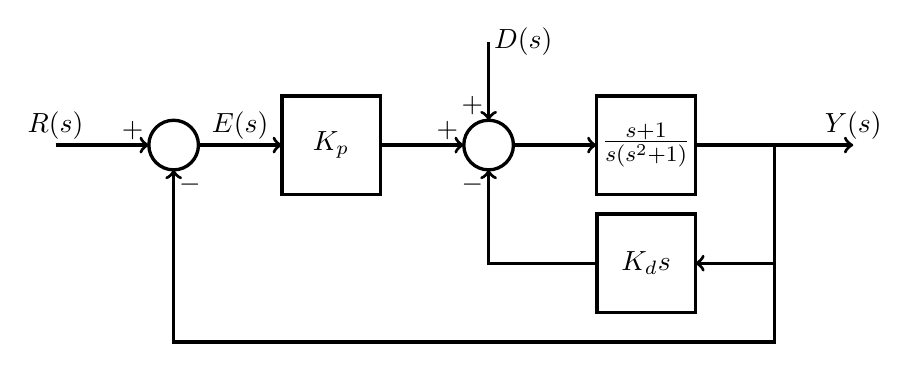
\begin{tikzpicture}[scale=1,inner sep=0pt,outer sep=0pt,very thick,
sysblock/.style={draw,rectangle,inner sep=2pt,minimum width=1.25cm,minimum height=1.25cm,very thick}]
\draw (1.5,0) node[draw,circle] (sum1) {$\rule{0pt}{18pt}$};
\draw (3.5,0) node[sysblock] (Kp) { $\large K_{p}$};
\draw (5.5,0) node[draw,circle] (sum2) {$\rule{0pt}{18pt}$};
\draw (7.5,0) node[sysblock] (G) {\large $\frac{s+1}{s(s^2+1)}$};
\draw (7.5,-1.5) node[sysblock] (Kd) {$K_{d}s$};
\draw[->] (0,0) node[above=2pt] {$R(s)$} -- (sum1.180) node[above left=2pt] {$+$};
\draw[->] (sum1.0) -- node[above=2pt] {$E(s)$} (Kp);
\draw[->] (Kp) -- (sum2.180) node[above left=2pt] {$+$};
\draw[->] (sum2.0) -- (G.180);
\draw[<-] (sum2.90) node[above left=2pt] {$+$} -- ++(0,1) node[right=2pt] {$D(s)$};
\draw[->] (G.0) -- ++(2,0) node[above=2pt] {$Y(s)$};
\draw[->] (G.0) ++(1,0) |- (Kd.0);
\draw[->] (Kd.180) -| (sum2.-90) node[below left=2pt] {$-$};
\draw[->] (G.0) ++(1,0) -- ++(0,-2.5) -| (sum1.-90) node[below right=2pt] {$-$};
\end{tikzpicture}
\end{center}
Here $r$ is a reference input, $y$ is the system output, $e$ is the error $e=r-y$ and $d$ is a disturbance. If $d(t)$ is a unit step, and $r(t)=0$, what is the steady state error $\lim_{t\rightarrow  \infty} e(t)$ as a function of the gains $K_{p}$ and $K_{d}$? 
